
In this section, we discuss our data sources and the necessary data munging steps we used in our study.
We compiled a dataset for 94 unique locations in South Carolina with precipitation, elevation, gage height, along with basin information, over a span of five years.
We primarily cover the collection of variables such as daily rainfall and gage height, since we are interested in exploring the dynamics between them.
We mention the watershed information briefly since it is used in defining the proximity matrix.
A detailed discussion of this can be found in Section~\ref{sec:watershed}.

\subsection{Precipitation}\label{subsec:precipitation}
The National Weather Service (NWS) collects precipitation data at 12 Contiguous United States (CONUS) River Forecast Centers (RFCs).
The precipitation is recorded using a multisensor approach.
Hourly estimates from weather radars are compared to ground gage reports, and a correction factor is calculated and applied to the radar field (Daly et al., 2001).
For areas where radar coverage is not accessible, satellite precipitation estimates can be used to construct the multisensor field (Daly et al., 1994).
Note that this method has been applied to South Carolina and most other eastern states, whereas a different method is used to process  precipitation data in mountainous areas west of the Continental Divide.\\

The precipitation data are then mosaicked into a gridded field with a spatial resolution of four by four kilometers.
The record is an accumulation of 24-hour periods and 1200 GMT is used as the ending time for a 24-hour total.
Spatially, the original dataset extends well beyond the U.S. border, most notably north of Washington and Idaho and west of Texas, in order to model rivers that flow into the United States.
However, only the observations within South Carolina and nearby states are retained in our study since the rainfall far outside the state is unlikely to have a major effect on flood gage heights in the short term.
Available data dates back to 2004 and still is actively updated by NWS. Rainfall values from 2012 to 2016 (inclusive) were retrieved for our study.  \\

The raw data are archived in \url{https://water.weather.gov/precip/archive/}.
The major challenges of handling this dataset are parsing the raw data (in NetCDF format) and filtering out values from  irrelevant regions and dates.
 Section~\ref{subsec:code_intro} is a brief introduction of our proposed approaches to streamline the data preprocessing steps by developing a Python library.


\subsection{Gage Height}\label{subsec:gage-height}
Gage height (also known as stage) is the height of the water in the stream above a reference point.
Gage height refers to the elevation of the water surface in the specific pool at the streamgaging station, not along the entire stream (USGS, 2011).
Gage height also is not exactly the same as the depth of the stream.
Since the stage baselines are set in a case-by-case manner across locations, we subtract the station-wise historical median (the median gage height for each location, over a 10-year period) from each gage height measurement to make the measurements comparable (see Section~\ref{sec:model}  for details).
This is done as a preliminary centering step before we fit the model.\\

The U.S. Geological Survey (USGS) provides an archive of approximately 1.9 million observation sites of all kinds in all 50 states,  the District of Columbia, Puerto Rico, the Virgin Islands, Guam, American Samoa, under the\emph{Water Data for the Nation} portal on its website.
More than 1000 such sites can be found within the border of South Carolina. However, the site count is drastically reduced when we focus on locations measuring surface water and exclude those that have ceased functioning. Eventually, we have approximately 150 to 200 locations (depending on the timeframe) within South Carolina that give a valid reading of the gage level on a daily basis. One can either use the interface provided by USGS or the \texttt{data.download\char`_flood()} function from our Python library (Section~\ref{subsec:code_intro}) to download the data. The former comes with a graphical user interface but may be harder to maneuver when multiple sites are needed. The latter, on the other hand, allows user customization to a greater degree. \\

Notably, the precipitation and the gage height are measured in different locations, since the former are measured  in gridded fields and the latter are located at major rivers and dams. We implemented a ``blurry lookup''  approach to  combine the two pieces of information. For readers familiar with SQL, the algorithm is similar to a left join, where all rows in the left table (gage height) are retained, and on the right (precipitation) only records with  matching keys are kept. This is different from a typical left join in that although a latitude and longitude pair serves as the key, typical merging is not feasible due to the location mismatch. Hence, the merging is done by finding  the nearest neighbor. For each row (location $ i$) in the gage height table, we find a location $ j$ in the precipitation table that is closest to it. We add the rainfall information at location $ j$ to location $ i$ for each $ i$ in the left table. Admittedly, this is not ideal since the precipitation and gage height are not from the exact same location, but the high resolution of the precipitation data ($ 4 \times 4 $ km) makes this issue less critical.\\

Additionally, since a fair amount of records are missing in the dataset, we first calculate the   missing data ratio, which is the percentage of days with missing records over the total number of days during the aforementioned time span (2012-2016). We discard the location if the missing data ratio is beyond a certain threshold. We strike a balance between a larger sample size and better data completeness with the help of Figure~\ref{missing_data}, which shows how many locations are retained for different time spans and thresholds. Note that the x-axis is number of years from 2016 counting backwards. For instance, there are 120 locations retained in the dataset for 2016 with a 95\% complete-data threshold. Based on Figure~\ref{missing_data}, we pick 90\% (94 unique stations) as the complete-data threshold for a time span of five years, since further increasing the threshold leads to a significant decrease in the amount of available gaging stations. \\

\begin{figure}[htbp]
\begin{center}
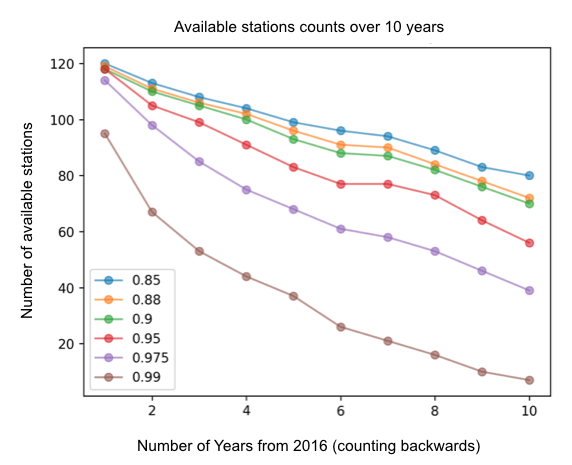
\includegraphics[width=0.6\textwidth]{../images/station_counts_by_year.png}
\caption{\hl{The number of available stations based on different complete-data thresholds.}}
\label{missing_data}
\end{center}
\end{figure}

Imputation for the remaining locations is based on the temporal adjacency. In other words, to fill the missing gage height values on certain dates, the weighted average of values from neighboring dates is used, that is
\begin{align*}
  Y_t = \frac{w_{t-2}}{w*} Y_{t-2} + \frac{w_{t-1}}{w*}Y_{t-1} + \frac{w_{t+1}}{w*}Y_{t+1} + \frac{w_{t+2}}{w*}Y_{t+2},
\end{align*} 

\noindent where $Y_t$  is the missing value at time $t$ and $ w* =w_{t-2} + w_{t-1}+ w_{t+1} + w_{t+2}$. We set $ w_{t-1} = w_{t+1} = 2$ and $ w_{t-2} = w_{t+2} = 1$ since  observations closer in time to the missing value should be more informative.
Alternatively, one can fill the missing values based on spatial closeness, but we argue that the gage height measurements in the \emph{same} location may change quite steadily and continuously. Filling missing data spatially is less ideal since doing so would involve pooling together different observation locations, which are associated with varying gage baseline levels and landscapes.


\subsection{Elevation}
The elevation information  is obtained based on the Shuttle Radar Topography Mission (SRTM), which is an international research effort that obtained digital elevation models on a near-global scale from 56$^\circ$S to 60$^\circ$N (Farr et al., 2007). The 30-meter topographic data products are  publicly distributed by the USGS along with the 90-meter data. These data are made available via an Earth Explorer on the US Geological Survey website in a \texttt{.tiff} format. We retrieve the elevation information from the 90-meter data for the aforementioned gage locations by matching the latitude and longitude. Elevation of the nearest neighbor is used if an exact match cannot be found. 


\subsection{Other Covariates}
Besides the precipitation and elevation, we also include three dummy variables to account for the seasonality in the data. The three dummy variables respectively take values 1 if the data record is from the spring (March through May), summer (June through August), or fall (September through November), and 0 otherwise. More importantly, interaction terms of the season indicator and precipitation are included, so that we can explore whether a difference in rainfall effect on flood levels exists across seasons. Specifically, if  the interaction variable between spring and precipitation manifests itself as  positive and significant, one can conclude that during March through May, rainfall increases are likely to lead to an even greater average rise in gage heights than in the baseline season (winter). 

\subsection{Basins and Watersheds}
The watershed information is pivotal to our model in a way that is different from elevation or precipitation. Rather than entering the model as a covariate, the watershed membership is used for the adjacency matrix $\bold W$, whose definition can be found in Section~\ref{sec:watershed}, along with a more detailed account of the watershed system. In this section, we focus  on preprocessing such information into a well-structured format. \\

USGS hosts the watershed information by state on Amazon Web Services (AWS), which is publicly available. It is a repository of contour files with varying sizes. A 4-digit hydrologic unit code (HUC) is less localized and covers a larger area \hl{than a 6-digit HUC (HUC-6), for example}. We use the contour information to define the watershed membership. Practically, a categorical variable with the watershed name is added for each available location. We decide to use the 6-digit hydrological unit to categorize all available locations into four regions.  We discuss this more in Section~\ref{sec:watershed}.

\subsection{Miscellaneous Code}\label{subsec:code_intro}
A Python library, \texttt{climate\char`\_data\char`\_toolkit}, is developed in parallel with our study, which accomplishes two goals.
First, we intend to streamline the process of downloading and preprocessing  raw data from different sources.
Rather than using varying user interfaces for different databases, one can achieve the same result nearly instantly by function calls like \texttt{get\char`\_flood()}.
Second, we package our models that we use in Section~\ref{sec:model} with a user-friendly interface. Hence, a compilation of a few Python modules, or, a library, is a natural choice for this purpose. In addition, we also have a plotting system, which is a handy tool to visualize spatial data, since it can display spatial elements such as markers and contours on top of an OpenStreet Map in a manner reminiscent of the R package \texttt{ggplot} (Wickham, 2019). The Python library is hosted on Github, and users can find the source code and help documents at \url{https://github.com/HaigangLiu/spatial-temporal-py}. Alternatively, the package also supports \texttt{pip install}, which is a convenient command line tool for package management.
